
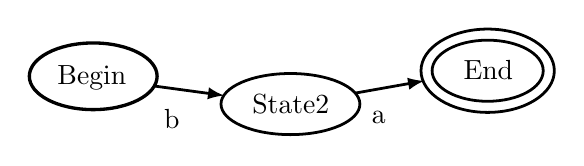
\begin{tikzpicture}[>=latex,line join=bevel,]
  \pgfsetlinewidth{1bp}
%%
\pgfsetcolor{black}
  % Edge: State2 -> End
  \draw [->] (119.39bp,18.958bp) .. controls (124.1bp,19.794bp) and (129.15bp,20.689bp)  .. (144.13bp,23.346bp);
  \definecolor{strokecol}{rgb}{0.0,0.0,0.0};
  \pgfsetstrokecolor{strokecol}
  \draw (127.76bp,10.265bp) node {a};
  % Edge: Begin -> State2
  \draw [->] (46.761bp,21.521bp) .. controls (51.538bp,20.872bp) and (56.693bp,20.173bp)  .. (72.11bp,18.082bp);
  \draw (53.283bp,9.5bp) node {b};
  % Node: State2
\begin{scope}
  \definecolor{strokecol}{rgb}{0.0,0.0,0.0};
  \pgfsetstrokecolor{strokecol}
  \draw (96bp,15bp) ellipse (25bp and 11bp);
  \draw (96.097bp,14.827bp) node {State2};
\end{scope}
  % Node: Begin
\begin{scope}
  \definecolor{strokecol}{rgb}{0.0,0.0,0.0};
  \pgfsetstrokecolor{strokecol}
  \draw [very thick] (25bp,25bp) ellipse (23bp and 12bp);
  \draw (24.5bp,24.541bp) node {Begin};
\end{scope}
  % Node: End
\begin{scope}
  \definecolor{strokecol}{rgb}{0.0,0.0,0.0};
  \pgfsetstrokecolor{strokecol}
  \draw (167bp,27bp) ellipse (20bp and 11bp);
  \draw (167bp,27bp) ellipse (24bp and 15bp);
  \draw (167.23bp,27.443bp) node {End};
\end{scope}
%
\end{tikzpicture}
